% !TEX program = pdflatex
\documentclass[11pt,a4paper]{article}

% --- packages (kept minimal and standard) ---
\usepackage[utf8]{inputenc}
\usepackage[T1]{fontenc}
\usepackage{lmodern}
\usepackage{geometry}
\geometry{margin=1in}
\usepackage{amsmath,amssymb}
\usepackage{siunitx}
\usepackage{graphicx}
\usepackage[font=small,labelfont=bf,labelsep=endash]{caption}
\usepackage{booktabs}
\usepackage{physics}
\usepackage{hyperref}
\hypersetup{colorlinks=true,linkcolor=blue,citecolor=blue,urlcolor=blue}

% --- title & author ---
\title{Design Methodology for a Dual-Jet Hovering Disc Using Concentric Air Curtains}
\author{ }
\date{ }

\begin{document}
\maketitle

\begin{abstract}
This work presents a physical model and an operational design methodology for a hovering disc sustained by two concentric air jets.
The outer annular jet forms an aerodynamic curtain that confines the inner flow and minimizes leakage, whereas the inner jet compensates the residual mass loss to maintain a controlled cushion pressure beneath the disc. The paper states the governing equations for lift balance, leakage through the peripheral gap, and curtain dynamics (momentum balance and flow split), and provides a step-by-step sizing procedure to achieve stable hovering with minimum power. Finally, a dedicated section shows the simulation outputs produced by the accompanying Python script, loading figures from a common directory.
\end{abstract}

\section{Introduction and Operating Principle}
The device is a rigid circular disc of radius $R$ hovering at a distance $h$ from the ground by sustaining a nearly uniform overpressure $p_c$ in the central cushion region. Two coaxial jets are employed (Fig.~\ref{fig:geometry}): an \emph{outer annular jet} (``corona'') acting as an air curtain that seals and recirculates the cushion flow, and an \emph{inner jet} that compensates for the residual mass leakage across the peripheral gap.
The design goal is to select geometry and jet operating points so that the target payload $W$ is carried with acceptable power and stability margins.

\section{Geometry and Notation}
We adopt the following notation, consistent with the schematic in Fig.~\ref{fig:geometry}:
\begin{itemize}
  \item $R$ disc radius; $w$ ring width of the leakage annulus near the rim ($R-w\le r\le R$);
  \item $h$ nominal clearance to the ground; $h_{\mathrm{eff}}$ effective leakage height at the rim (may be smaller than $h$ due to the curtain and flow turning);
  \item $p_c$ cushion overpressure (assumed uniform);
  \item Outer jet (\textit{corona}): mass flow $\dot m_{\mathrm{corona}}$, slot thickness $b$, slot area $A_{\mathrm{corona}}=2\pi R\,b$, exit speed $U_{\mathrm{corona}}=\dot m_{\mathrm{corona}}/(\rho A_{\mathrm{corona}})$;
  \item Inner jet: mass flow $\dot m_{\mathrm{in}}$;
  \item Mass loss from the cushion across the periphery: $\dot m_{\mathrm{loss}}$; volumetric loss $Q_{\mathrm{loss}}=\dot m_{\mathrm{loss}}/\rho$.
\end{itemize}
\begin{figure}[t]
  \centering
  % Note: figures are loaded from ../figs/ as per repository layout
  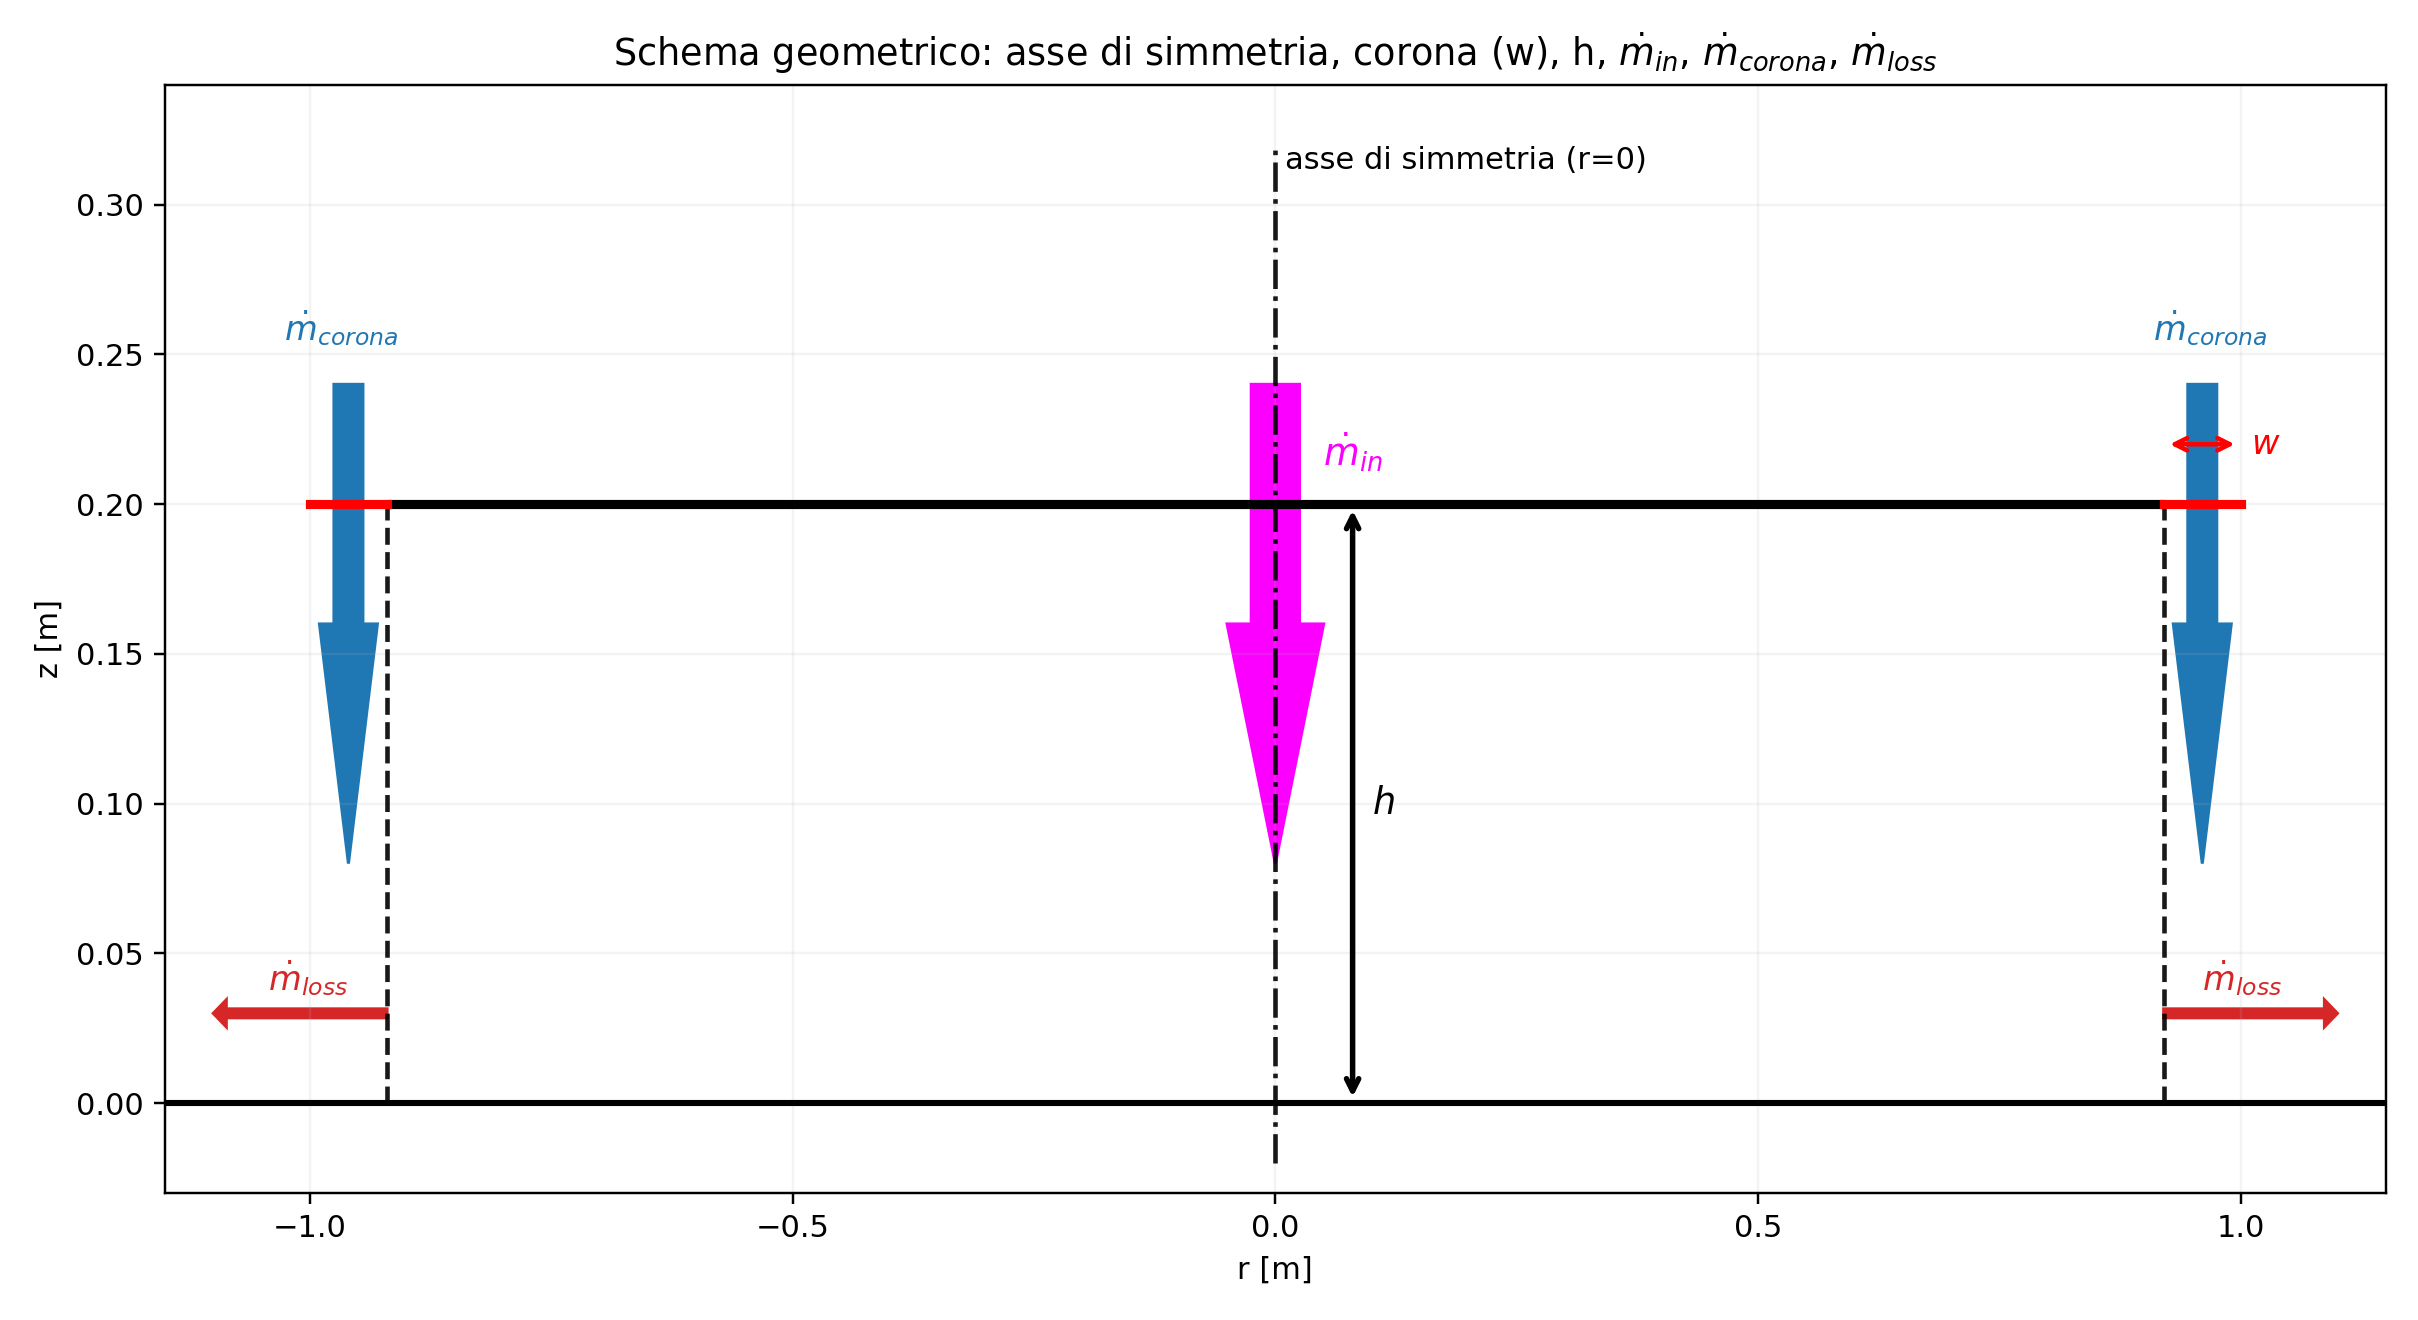
\includegraphics[width=0.95\linewidth]{../figs/schema_geometry.png}
  \caption{Geometric scheme (axes of symmetry, annulus width $w$, hover height $h$) and the two concentric jets: inner make-up flow $\dot m_{\mathrm{in}}$ and outer annular jet $\dot m_{\mathrm{corona}}$ forming the air curtain that reduces leakage $\dot m_{\mathrm{loss}}$.}
  \label{fig:geometry}
\end{figure}

\section{Lift Balance}
The hovering condition is set by the pressure force over the planform area:
\begin{equation}
  p_c\,\pi R^2 = W
  \quad \Rightarrow \quad
  p_c = \frac{W}{\pi R^2}.
  \label{eq:lift}
\end{equation}
Equation~\eqref{eq:lift} defines the target cushion pressure for a given payload.

\section{Leakage Through the Peripheral Gap}
The peripheral annulus governs the mass loss $\dot m_{\mathrm{loss}}$. Two regimes are considered; the applicable model is selected based on the local Reynolds number $\mathrm{Re}_h=\rho U_h h_{\mathrm{eff}}/\mu$, with $U_h\approx Q_{\mathrm{loss}}/(2\pi R h_{\mathrm{eff}})$.

\subsection*{Viscous (lubrication) regime}
\begin{equation}
  Q_{\mathrm{loss}}
  = \frac{\pi h_{\mathrm{eff}}^{3}\,p_c}{6\,\mu\,\ln\!\big(\tfrac{R}{R-w}\big)},
  \qquad \dot m_{\mathrm{loss}}=\rho\,Q_{\mathrm{loss}}.
  \label{eq:qloss_lub}
\end{equation}

\subsection*{Inertial (orifice) regime}
Let $A_{\mathrm{eff}}=2\pi R\,h_{\mathrm{eff}}$:
\begin{equation}
  Q_{\mathrm{loss}}
  = C_d\,A_{\mathrm{eff}}\,\sqrt{\frac{2\,p_c}{\rho}},
  \qquad \dot m_{\mathrm{loss}}=\rho\,Q_{\mathrm{loss}}.
  \label{eq:qloss_orif}
\end{equation}
In transitional conditions a smooth interpolation between \eqref{eq:qloss_lub} and \eqref{eq:qloss_orif} can be used.

\section{Air-Curtain (Outer Jet) Dynamics}
The outer annular jet is turned near the rim and forms a wall-jet that seals the cushion.
A momentum balance across a thin control volume of height $h_{\mathrm{eff}}$ at the rim gives the curtain condition
\begin{equation}
  p_c \simeq C_t\,\frac{\rho U_{\mathrm{corona}}^{2} \, b}{h_{\mathrm{eff}}},
  \label{eq:curtain_force}
\end{equation}
where $C_t=\mathcal{O}(1)$ collects turning and wall-jet losses.
It is convenient to define the nondimensional momentum ratio
\begin{equation}
  J\;\equiv\; \frac{\rho U_{\mathrm{corona}}^{2}\,b}{p_c\,h_{\mathrm{eff}}}
  \quad \text{with} \quad J\gtrsim J_{\min}=1/C_t.
  \label{eq:J}
\end{equation}
Given $J$ (design margin), the required outer-jet speed and mass flow follow from $U_{\mathrm{corona}}=\sqrt{J\,p_c h_{\mathrm{eff}}/(\rho b)}$ and
\begin{equation}
  \dot m_{\mathrm{corona}} = \rho\,A_{\mathrm{corona}}\,U_{\mathrm{corona}}
  = 2\pi R\,\rho\,b\,\sqrt{\frac{J\,p_c h_{\mathrm{eff}}}{\rho b}}
  = 2\pi R\,\sqrt{\rho\,p_c}\; b\,\sqrt{\frac{J h_{\mathrm{eff}}}{b}}.
  \label{eq:mcorona}
\end{equation}

\subsection*{Flow split of the outer jet}
The wall-jet entrains fluid on both sides.
A fraction $\beta\in[0,1]$ of $\dot m_{\mathrm{corona}}$ turns inward and reinforces the cushion; the remainder leaves outward:
\begin{equation}
  \dot m_{\mathrm{rein}}=\beta\,\dot m_{\mathrm{corona}},\qquad
  \dot m_{\mathrm{out}}=(1-\beta)\,\dot m_{\mathrm{corona}}.
  \label{eq:split}
\end{equation}
In design, $\beta$ may be treated as a function of the curtain strength and geometry.
A practical closed form, to be calibrated, is
\begin{equation}
  \beta = \frac{1}{1+\gamma\,(h_{\mathrm{eff}}/b)\,J^{-1/2}},\qquad \gamma=\mathcal{O}(1),
  \label{eq:beta}
\end{equation}
which increases towards unity as the curtain becomes stronger (larger $J$) and the slot is thinner.

\section{Cushion Mass Balance and Make-Up Flow}
Assuming a well-mixed cushion, stationarity requires
\begin{equation}
  \dot m_{\mathrm{in}} + \dot m_{\mathrm{rein}} = \dot m_{\mathrm{loss}}
  \quad \Rightarrow \quad
  \boxed{\ \dot m_{\mathrm{in}} = \dot m_{\mathrm{loss}} - \beta\,\dot m_{\mathrm{corona}}\ }.
  \label{eq:massbalance}
\end{equation}

\section{Power Estimates}
The ideal aerodynamic power is the sum of the cushion power and the jet kinetic power:
\begin{equation}
  P_{\mathrm{ideal}} \approx p_c\,Q_{\mathrm{loss}} + \frac{\dot m_{\mathrm{corona}}\,U_{\mathrm{corona}}^{2}}{2}.
  \label{eq:power}
\end{equation}
With overall efficiency $\eta$ (blower + ducts), the shaft/electrical power is $P=P_{\mathrm{ideal}}/\eta$.

% ------------------------------------------------------------------
\section{Simulation Outputs}
This section loads the figures saved by the Python script \texttt{scripts/run\_sim.py} into the shared directory \texttt{../figs/}.
Each figure includes a vertical line at $r=R^-=R-w$ as a visual reference.

\begin{figure}[t]
  \centering
  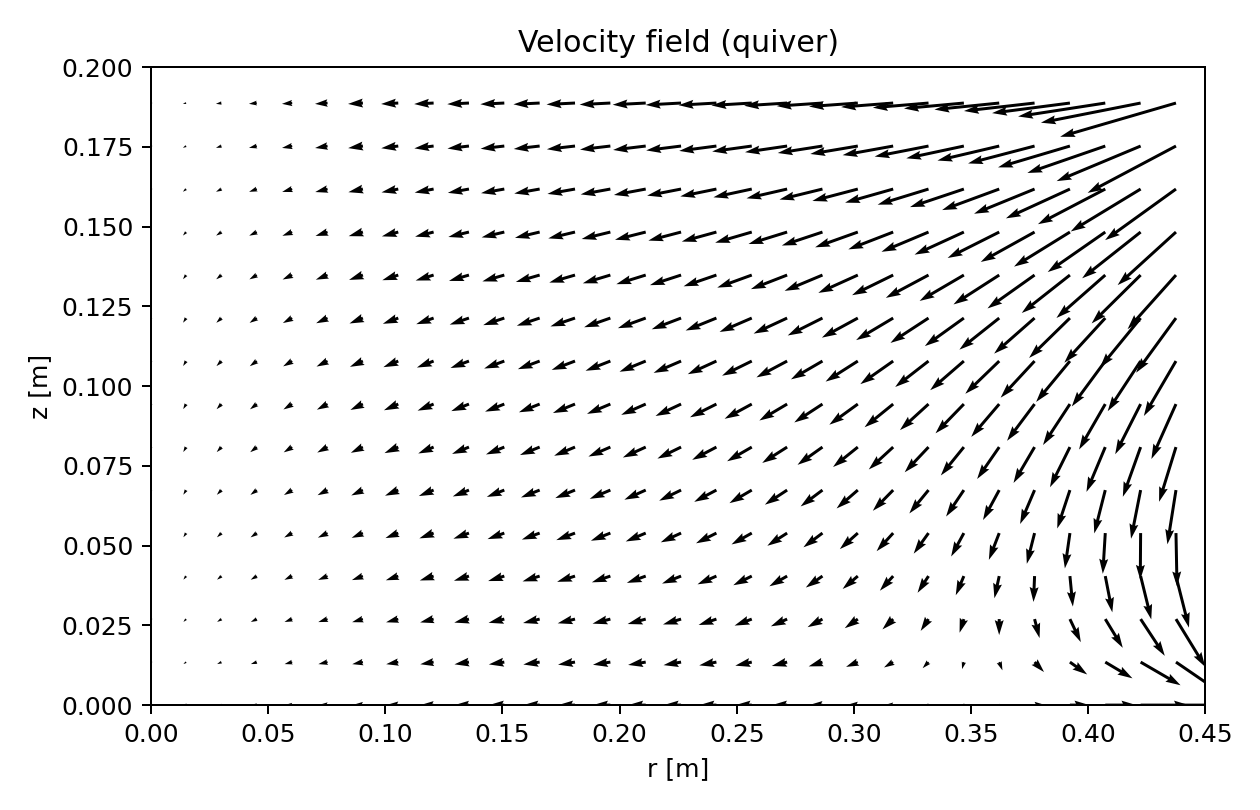
\includegraphics[width=0.95\linewidth]{../figs/quiver_velocity.png}
  \caption{Velocity field (quiver) over the $(r,z)$ domain; downward vertical components (negative $z$) reflect the purely vertical jet condition at $z=h$.}
  \label{fig:quiver}
\end{figure}

\begin{figure}[t]
  \centering
  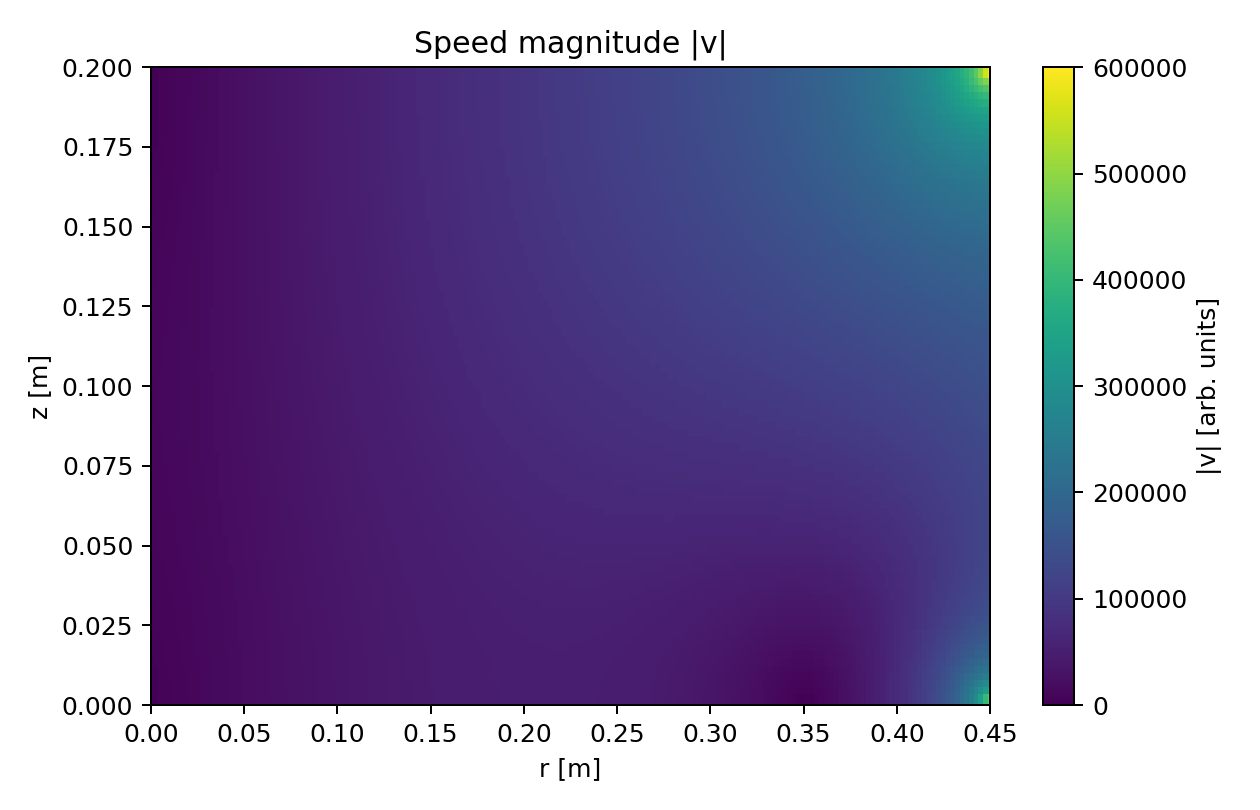
\includegraphics[width=0.95\linewidth]{../figs/cmap_speed.png}
  \caption{Colormap of speed magnitude $\lvert \mathbf{v}\rvert$.}
  \label{fig:cmap_speed}
\end{figure}

\begin{figure}[t]
  \centering
  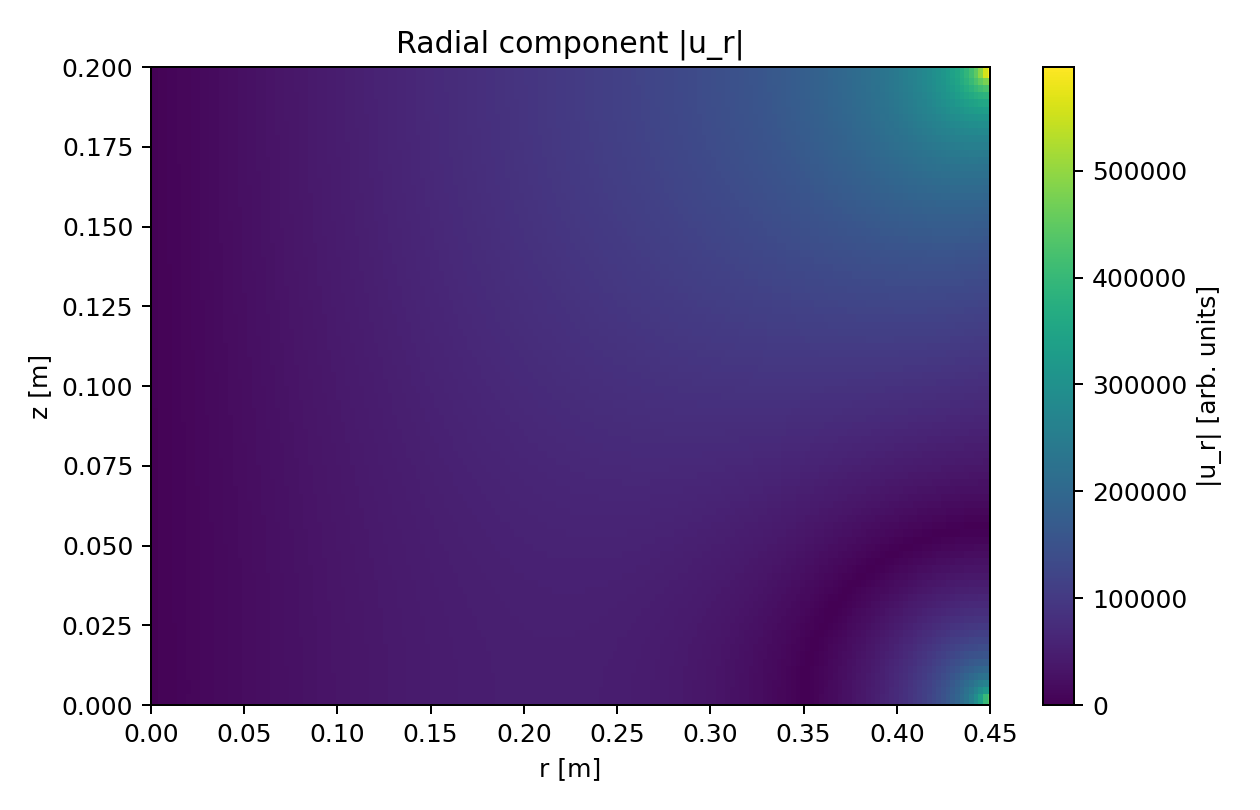
\includegraphics[width=0.95\linewidth]{../figs/cmap_ur.png}
  \caption{Colormap of radial component magnitude $\lvert u_r\rvert$.}
  \label{fig:cmap_ur}
\end{figure}

\begin{figure}[t]
  \centering
  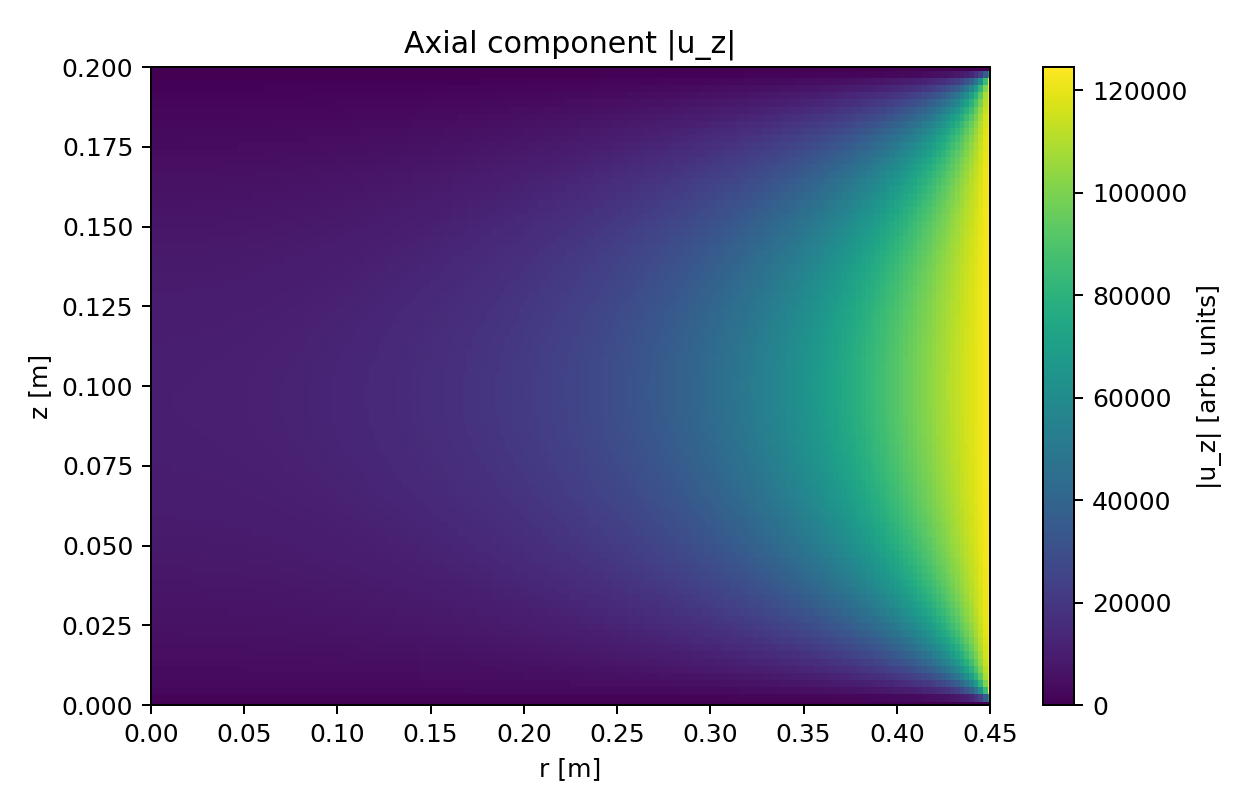
\includegraphics[width=0.95\linewidth]{../figs/cmap_uz.png}
  \caption{Colormap of axial component magnitude $\lvert u_z\rvert$.}
  \label{fig:cmap_uz}
\end{figure}

\begin{figure}[t]
  \centering
  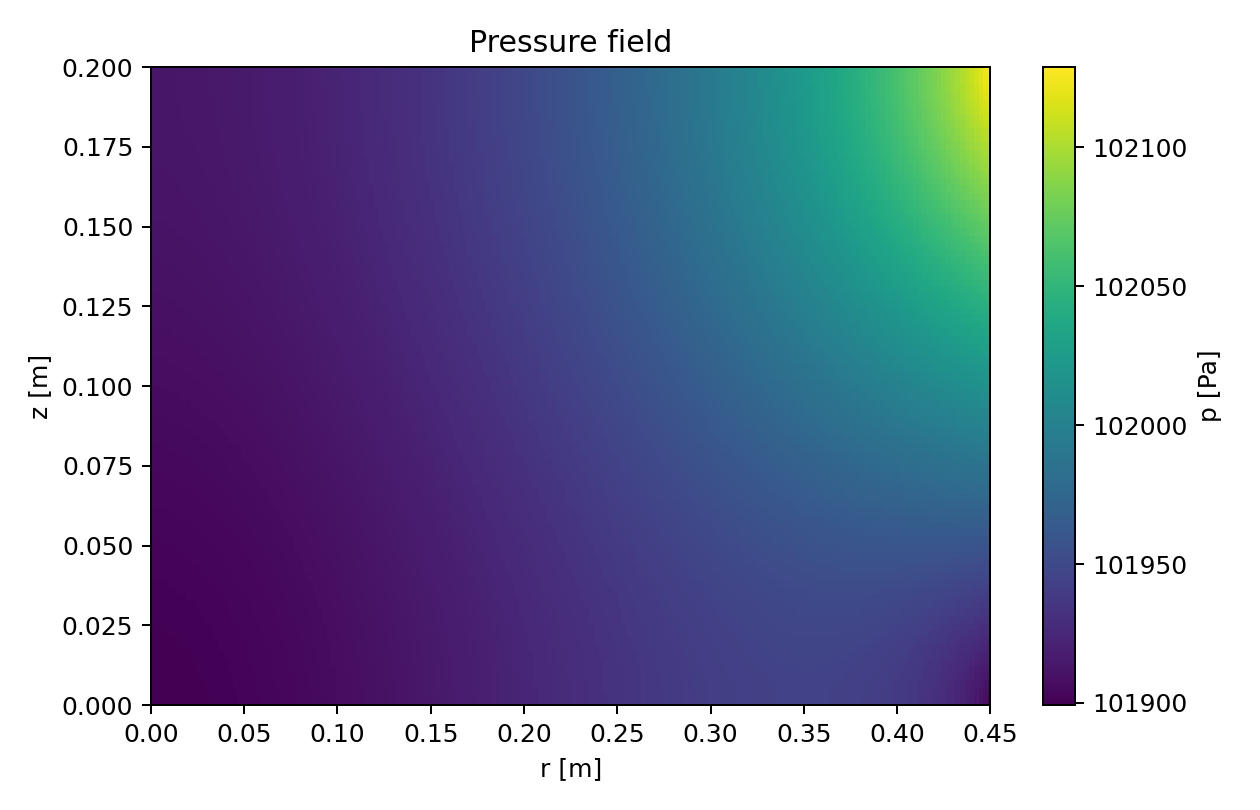
\includegraphics[width=0.95\linewidth]{../figs/cmap_pressure.png}
  \caption{Colormap of pressure $p(r,z)$.}
  \label{fig:cmap_p}
\end{figure}

\end{document}
